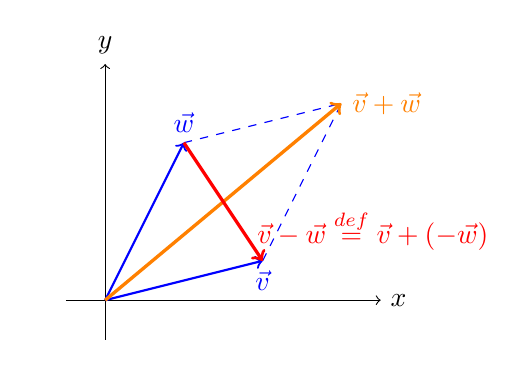
\begin{tikzpicture}
    %draw lines
    \draw [->] (-0.5,0) -- (3.5,0) node[right]{$x$};
    \draw [->] (0,-0.5) -- (0,3) node[above]{$y$};
    \draw [-,blue,dashed] (1,2) -- (3,2.5);
    \draw [-,blue,dashed] (2,0.5) -- (3,2.5);
    \draw [->,blue,thick] (0,0) -- (2,0.5) node[below]{$\vec{v}$};
    \draw [->,blue,thick] (0,0) -- (1,2) node[above]{$\vec{w}$};
    \draw [->,orange,very thick] (0,0) -- (3,2.5) node[right]{$\vec{v}+\vec{w}\hspace{0.5cm}$};
    \draw [->,red,very thick] (1,2) -- (2,0.5) node[above]{$\hspace{28mm}\vec{v}-\vec{w}\stackrel{def}{=}\vec{v}+(-\vec{w})$};
\end{tikzpicture}
\captionof{figure}{{\footnotesize vector head-to-tail operation.}}
\label{fig:vector-and-vector-operation-d4}
